\documentclass{article}

\usepackage{neurips_2019}

\usepackage[utf8]{inputenc} % allow utf-8 input
\usepackage[T1]{fontenc}    % use 8-bit T1 fonts
\usepackage[pdfborder={0 0 0}]{hyperref}       % hyperlinks
\usepackage{url}            % simple URL typesetting
\usepackage{booktabs}       % professional-quality tables
\usepackage{amsfonts}       % blackboard math symbols
\usepackage{nicefrac}       % compact symbols for 1/2, etc.
\usepackage{microtype}      % microtypography

\usepackage{subcaption}
\usepackage{graphicx}
\usepackage{amsmath}
\usepackage{amssymb}
\usepackage{bm}
\usepackage{relsize}
\usepackage{natbib}
\usepackage{float}
\usepackage{tikz}

\usetikzlibrary{shapes,arrows}

\tikzstyle{block} = [rectangle, draw, thick, align=center, rounded corners]
\tikzstyle{boundingbox} = [very thick, dotted, gray]
\tikzstyle{dashblock} = [rectangle, draw, thick, align=center, dashed]
\tikzstyle{conc} = [ellipse, draw, thick, dashed, align=center]
\tikzstyle{netnode} = [circle, draw, very thick, inner sep=0pt, minimum size=0.5cm]
\tikzstyle{relunode} = [rectangle, draw, very thick, inner sep=0pt, minimum size=0.5cm]
\tikzstyle{line} = [draw, very thick, -latex']

\setlength{\parskip}{1em}
\setlength{\parindent}{0em}

\setcitestyle{square}

\begin{document}
\title{Embedded Meta-Learning: Toward more flexible deep-learning models}
\author{Andrew K. Lampinen}
\date{}
\maketitle

\section{Introduction}
Humans are able to use and reuse knowledge more flexibly than most deep learning models can \citep[e.g.][]{Lake2016}. One fundamental reason for this is that humans are aware of what we are trying to compute and why. By contrasts, there is a fundamental separation of knowledge within most deep neural networks -- although deep networks represent knowledge about data (in their activations) and knowledge about the structure of tasks (in their parameters), they do not represent any relationships between data and tasks. That is, neural networks knowledge about what is being computed is only implicitly accessible to those computations. \par
There are a number of advantages to representing knowledge about data and tasks. In particular, it can grant the ability to rapidly adapt behavior to a new task. The problem of rapid learning has been partially addressed by meta-learning systems \citep[e.g.][]{Vinyals2016, Finn2017a}. However, humans can take our knowledge and flexibly alter our behavior in accordance with a change in task demands or a single instruction. For example, once we learn to play a game, we can immediately switch to playing in order to lose, and can achieve reasonable performance without any retraining (i.e. zero-shot). Deep learning systems at present generally lack this representational flexiblity. \par
In this paper, we propose a new class of architectures which essentially take a functional perspective on meta-learning and exploit the idea of homoiconicity\footnote{A homoiconic programming language is one in which programs in the language can be manipulated by programs in the language, just as data can.}. By treating tasks and data as functions, we can conceptually think of both data \emph{and} learned behaviors as transformable. This yields the ability to not only learn to solve new tasks, but to learn how to flexibly transform these solutions in response to changing task demands. We suggest that this ability will be key to building more intelligent and flexible deep learning systems. \par
In particular, we propose a meta-learning architecture which embeds data (including natural language inputs) and tasks in a shared space, and meta-learns to execute mappings over this space. We demonstrate that this approach allows flexible remapping of behavior, as well as offering other benefits such as a useful framework for continual learning. \par
\section{Method}
\subsection{Architecture}
The essential idea of the architecture is that we separate the system into two parts: 
\begin{enumerate}
\item Domain specific encoders and decoders (vision, language, etc.) that map into a shared embedding space $Z$.
\item A meta-learning system which:
    \begin{enumerate}
    \item Embeds tasks into the shared embedding space $Z$.
    \item Learns to perform tasks in accordance with their embeddings.
    \end{enumerate}
\end{enumerate}
The utility of having a completely shared space $Z$ in which data, language, and tasks are represented is that it allows for arbitrary mappings between these distinct types of data. In addition to basic tasks, the system could in principle learn to map language to tasks (follow instructions) or tasks to language (explaining behavior), or tasks to tasks (changing behavior). This is a step closer to the flexible reasoning humans display. \par
Without training on these mappings, of course, the system will not be able to execute them well. However, ideally if it is trained on a braod enough set of such mappings, it will be able to generalize these to new instances drawn from the same data/task distribution. For instances that fall outside its data distribution or for optimal performance it may require some retraining. This reflects the structure of human behavior -- we are able to learn rapidly when new knowledge is relatively consistent with our previous knowledge, but learning an entirely new paradigm (such as calculus for a new student) can be quite slow. \par 
\begin{figure}
\centering
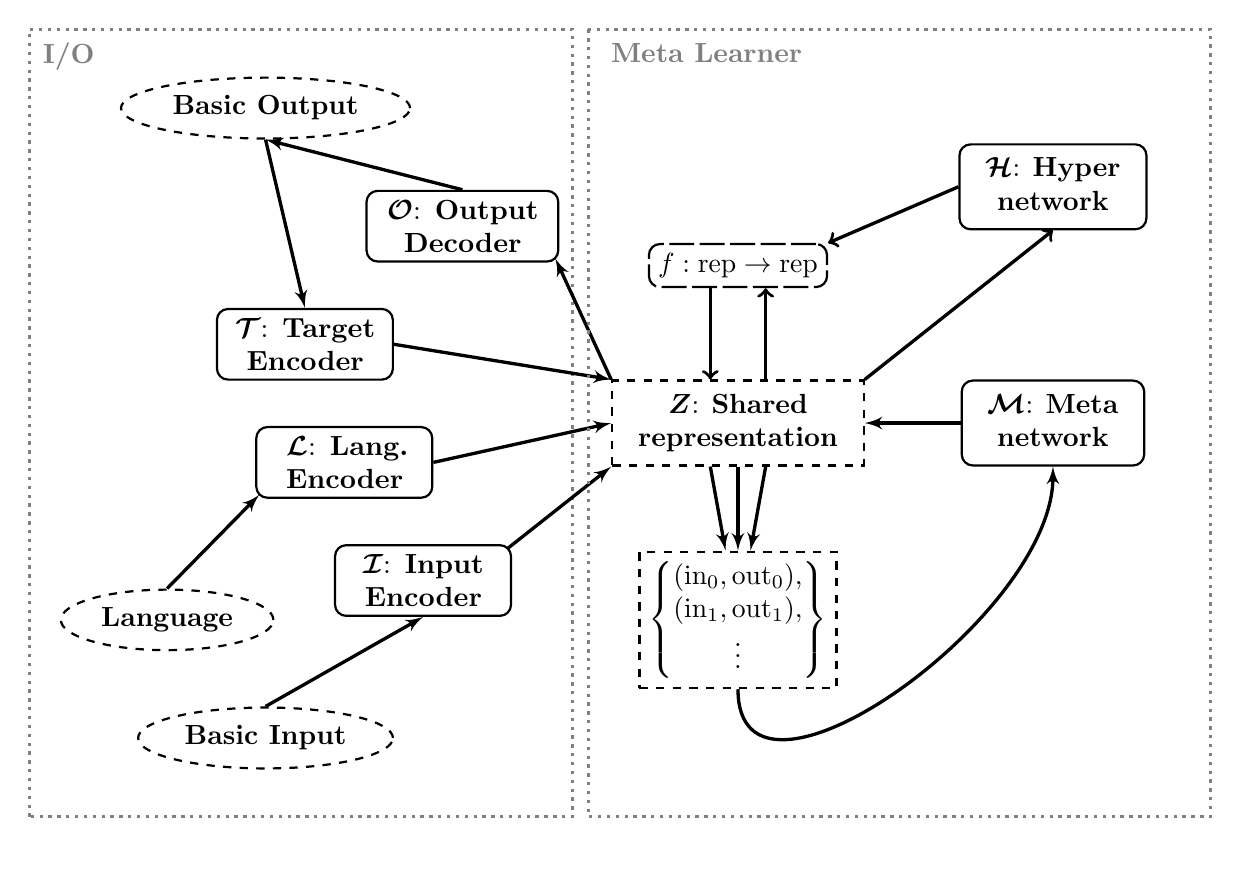
\begin{tikzpicture}[auto]

\node [dashblock] at (0, 0) (rep) {\begin{tabular}{c}$\bm{Z}$: \textbf{Shared} \\ \textbf{representation}\end{tabular}};

% inputs, outputs

\draw [boundingbox] (-9, -5) rectangle (-2.1, 5); 
\node [text=gray] at (-8.5, 4.65) {\textbf{I/O}};

\node [conc] at (-6, -4) (perc) {\textbf{Basic Input}};
\node [conc] at (-7.25, -2.5) (lang) {\textbf{Language}};
\node [conc] at (-6, 4) (act) {\textbf{Basic Output}};
\node [block, text width=2cm] at (-4, -2) (IE) {$\bm{\mathcal{I}}$: \textbf{Input Encoder}};
\node [block, text width=2cm] at (-5, -0.5) (LE) {$\bm{\mathcal{L}}$: \textbf{Lang. Encoder}};
\node [block, text width=2.2cm] at (-3.5, 2.5) (OD) {$\bm{\mathcal{O}}$: \textbf{Output Decoder}};
\node [block, text width=2cm] at (-5.5, 1) (TE) {$\bm{\mathcal{T}}$: \textbf{Target Encoder}};
\path [line] (perc.north) to (IE.south);
\path [line] (lang.north) to ([xshift=0.05cm, yshift=0.05cm]LE.south west);
\path [line] ([xshift=-0.05cm, yshift=-0.05cm]IE.north east) to (rep.south west);
\path [line] (LE.east) to (rep.west);
\path [line] (rep.north west) to ([xshift=-0.05cm, yshift=0.05cm]OD.south east);
\path [line] (OD.north) to (act.south);
\path [line] (act.south) to (TE.north);
\path [line] (TE.east) to (rep.north west);

% meta
\draw [boundingbox] (-1.9, 5) rectangle (6, -5); 
\node [text=gray] at (-0.4, 4.7) {\textbf{Meta Learner}};

\node [dashblock] at (0, -2.5) (collection) {
\(\left\{
\begin{matrix}
(\text{in}_0, \text{out}_0),\\
(\text{in}_1, \text{out}_1),\\
$\vdots$
\end{matrix}\right\}\)};
\path [line] (rep.south) to (collection);
\path [line] ([xshift=-1em]rep.south) to (collection);
\path [line] ([xshift=1em]rep.south) to (collection);

\node [block] at (4, 0) (meta) {\begin{tabular}{c}$\bm{\mathcal{M}}$: \textbf{Meta} \\ \textbf{network}\end{tabular}};
\path [line] (collection.south) to [out=-90, in=-90] (meta.south);
\path [line] (meta.west) to (rep.east);

% hyper

\node [block] at (4, 3) (hyper) {\begin{tabular}{c}$\bm{\mathcal{H}}$: \textbf{Hyper} \\ \textbf{network}\end{tabular}};
\node [block, dash pattern=on 9pt off 2pt] at (0, 2) (transform) {\(f: \text{rep} \rightarrow \text{rep}\)};

\path [draw, ->, very thick] (rep.north east) to (hyper.south);
\path [draw, ->, very thick] (hyper.west) to (transform.north east);
\path [draw, ->, very thick] ([xshift=-1em]transform.south) to ([xshift=-1em]rep.north);
\path [draw, ->, very thick] ([xshift=1em]rep.north) to ([xshift=1em]transform.south);

\end{tikzpicture}
\caption{Schematic of our general architecure. Blocks with solid edges denote deep networks with learnable parameters, dashed edges represent inputs, outputs, embeddings, etc., and $f$ is a deep network with parameters specified by $\mathcal{H}$.} \label{architecture_fig}
\end{figure}
More formally, we take a \emph{functional} perspective on learning. A datum can be represented by a constant function which outputs it. (For example, each point in the latent space of an autoencoder can be thought of this way.) This allows us to interpret model inputs or outputs as functions. \par
We can then interpret most machine learning tasks as a mapping of functions to functions. These functions could represent data\footnote{Where ``data'' is a quite flexible term. The approach is relatively agnostic to whether the learning is supervised or reinforcement learning, whether inputs are images or natural language, etc.}, or they could be functions that operate on functions themselves. Under this perspective, learning tasks and learning to flexibly map between tasks, or learning to map from language to tasks, are all the same type of problem. \par
Specifically, we embed inputs, targets, and mappings into a shared representational space $Z$. Inputs are embedded by a deep network $\mathcal{I}: \text{input} \rightarrow Z$. Outputs are decoded from the representational space by a deep network $\mathcal{O}: Z \rightarrow \text{output}$. Targets are encoded by a deep network $\mathcal{T}: \text{targets} \rightarrow Z$. (Targets do not necessarily need to be output-like, e.g. in our RL tasks, we use (action, outcome) tuples as ``targets.'') \par
Given this, the task of mapping inputs to outputs can be framed as trying to find a transformation of the representational space that takes the (embedded) inputs from the training set to the (embedded) targets. These transformations are performed by a system with the following components:  
\begin{itemize}
\item $\mathcal{M}: \{(Z, Z), ...\} \rightarrow Z $ -- the meta network, which takes a set of (input embedding, target embedding) pairs and produces a function embedding. 
\item $\mathcal{H}: Z \rightarrow \text{parameters}$ -- the hyper network, which takes a function embedding and produces a set of parameters. 
\item $f: Z \rightarrow Z$ -- the transformation, implemented by a deep network with parameters specified by $\mathcal{H}$.
\end{itemize}
See Fig. \ref{architecture_fig} for a schematic of the architecture. \par 

\subsection{Operation}
A basic forward pass through the system might look as follows.
\begin{enumerate}
\item A training dataset of (input, target) pairs is embedded by $\mathcal{I}$ and $\mathcal{T}$ to produce a set of paired embeddings. Another set of (possibly unlabeled) inputs is provided and embedded.
\item The meta network $\mathcal{M}$ maps the set of embedded (input, target) pairs to a function embedding.
\item The hyper network $\mathcal{H}$ maps the function embedding to parameters for $f$, which is used to transform the second set of inputs to a set of output embeddings.
\item The output embeddings are decoded by $\mathcal{O}$ to produce a set of outputs.
\end{enumerate}
To write this explicitly, suppose we have some dataset of input, target pairs ($D_1 = \{(x_0, y_0), ...\}$), and some input $x$ for which we wish to generate a predicted output $\hat{y}$. This output would be generated as follows: 
\[\hat{y} = \mathcal{O}\left(f_{D_1}\left(\mathcal{I} \left(x\right)\right) \right)\]
where $f_{D_1}$ is the transformation the meta-learner guesses for the training dataset $D_1$:
\[f_{D_1} \text{ is parameterized by } \mathcal{H}\left(\mathcal{M}\left( \left\{\left(\mathcal{I}\left(x_0\right), \mathcal{T}\left(y_0\right) \right), \left(\mathcal{I}\left(x_1\right), \mathcal{T}\left(y_1\right) \right), ... \right\}\right)\right)\]
This system can be trained end-to-end if labels are provided for a second set of inputs. In particular, suppose we have some loss function $\mathcal{L}(y, \hat{y})$ defined on a single target output $y$ and actual model output $\hat{y}$, for some input $x$. We define our total loss computed on some dataset $D_2$ as:
\[\mathbb{E}_{(x, y)\in {D}_2} \left[ \mathcal{L}\left(y, \mathcal{O}\left(f_{D_1}\left(\mathcal{I} \left(x\right)\right) \right)\right)\right]\]
More generally, suppose we have some input which is already embedded in the representation space $z_{in} \in Z$, and an embedded dataset $D_Z$ of (embedding, target embedding) pairs $\{(z_{in,0}, z_{out,0})\}$. Then we can generate an output $\hat{z}_{out} \in Z$ as:  
\[\hat{z}_{out} = f_{D_Z}(z_{in}) \qquad \text{where } f_{D_Z} \text{ is parameterized by } \mathcal{H}\left(\mathcal{M}\left(D_Z\right)\right)\]
This output can then be appropriately dispatched depending on the task at hand. For example, if the $z_{in,i}$ are the system's embeddings for trying to win various games, and the $z_{out,i}$ are the corresponding embeddings for trying to lose those games, then $z_{out}$ could be interpreted as the system's guess at a losing strategy for the game embedded as $z_{in}$, and then could be used to play that game. We could then evaluate performance by how well the system actually performs at losing with the $z_{out}$ strategy. \par
Similarly, we could map from language to a task embedding, and then ask how well the system performs at the task specified by language. The key feature of our architecture -- the fact that tasks, data, and language are all embedded in a shared space -- allows substantial flexibility within a unified system. 

\section{Experiments}
%\subsection{Boolean functions}
%As a proof of concept, we first evaluated the system on a simple task of computing boolean functions on boolean inputs. Specifically, we can imagine mapping from binary-valued input vectors to a single binary output representing the evaluation of some logical proposition on the input. We train the system to figure out how to compute the predicate from seeing a subset of the (input, output) pairs. \par   
%We can then train the system to do various meta-mappings, for example identifying certain types of functions (like XOR) or negating predicates. \par
%
\subsection{Learning multivariate polynomials}
\begin{figure}
\centering
\includegraphics[width=0.5\textwidth]{figures/poly/basic_results.png}
\caption{Basic meta-learning successfully generalizes to held out tasks. The solid line indicates optimal performance.}
\label{poly_basic_results}
\end{figure}

\begin{figure}
\centering
\includegraphics[width=0.75\textwidth]{figures/poly/meta_results.png}
\caption{The system generalizes to apply learned meta-mappings to new tasks, and to apply unlearned meta-mappings from seeing examples. The solid line indicates optimal performance.} 
\label{poly_meta_map_results}
\end{figure}
As a proof of concept, we first evaluated the system on the simple task of learning polynomials in 4 variables of degree $\leq 2$ (i.e. the task was to learn functions of the form $f: \mathbb{R}^4 \rightarrow \mathbb{R}$ where $f \in \mathcal{P}_2 \left(\mathbb{R}\right)$). This yields an infinite family of base-level tasks (the vector space of all such polynomials), as well as many families of meta-mappings over tasks (for example, multiplying a polynomial by a constant, squaring a polynomial, or permuting its input variables). This allows us to not only examine the ability of the system to learn to learn polynomials from data, but also to adapt its learned representations in accordance with these meta-tasks. \par

\textbf{Basic meta learning:} First, we show that the system is able to achieve the basic goal of learning a held-out task from a few examples in Fig. \ref{poly_basic_results}. \par 

\textbf{Meta mapping (task $\rightarrow$ task):} Furthermore, the system is able to perform meta-mappings (mappings over tasks) in order to flexibly reconfigure its behavior, as shown in fig. \ref{poly_meta_map_results}. We train the system to perform a variety of mappings, for example switch the first two inputs of the polynomial, add 3 to the polynomial, or square the polynomial. We then test its ability to generalize to held-out mappings, for example a permutation of the polynomial inputs which it has not encountered before, or an additive shift in the polynomial which it has not been trained on. The system is both able to apply its learned meta-mappings to held-out tasks, and to apply meta-mappings it has not been trained on, simply by seeing examples of their application. \par 


\subsection{Continual learning}
\begin{figure}
\centering
\includegraphics[width=\textwidth]{figures/continual/continual_learning.png}
\caption{Once the meta-learning system has been trained on a distribution of prior tasks, its performance on new tasks can be tuned by caching its guessed embeddings for the tasks and then optimizing those, thus avoiding any possibility of interfering with performance on prior tasks. Starting from random embeddings in the trained model results in slower convergence, while in an untrained model the embeddings cannot be optimized well.}
\label{poly_continual_results}
\end{figure}
Although the meta-learning approach is effective for rapidly adapting to a new task, it is unreasonable to think that our system must consider every example of a task it has seen at each inference step. We would like to be able to store our knowledge about the tasks in a way that allows it to be more carefully refined. Furthermore, we would like the system to be able to adapt to new tasks (that it cannot perfectly solve from examples) without catastrophically interfering with our prior knowledge \citep{McCloskey1989}. \par
A very simple solution to these problems is naturally suggested by our architecture. Specifically, task embeddings can be cached so that they don't have to be regenerated at each inference step. This also allows the potential to optimize these embeddings without altering the other parameters in the architecture, thus allowing fine-tuning on a task without seeing more examples, and without interfering with performance on any other task. That is, we can see the meta-learning step as a ``warm start'' for an optimization procedure over embeddings that are cached in memory \citep[c.f.][]{Kumaran2016}.\footnote{Note that the weights generated by the hyper network could be cached instead of the embeddings, which would be much more memory intensive but would allow even better tuning and would not require passing through the hyper network at inference time.} \par 
To test this idea, we pre-trained the system on 100 polynomial tasks, and then introduced 100 new tasks. We trained on these new tasks by starting from the meta-learning network's ``guess'' at the correct task embedding, and then optimizing this embedding without altering the other parameters. The results are shown in fig. \ref{poly_continual_results}. The meta-network embeddings offers good immediate performance, and substantially accelerates the optimization the process, compared to a randomly-initialized embedding. Furthermore, this ability to learn is due to training, not simply the expressiveness of the architecture, as is shown by attempting the same with an untrained network. \par 


\subsection{A stochastic learning setting: simple card games}
Our next case study was in the setting of simple card games, where the agent receives a hand and has to decide on a bet. There is no action besides betting, and depending on the opponent's hand the agent either wins or loses the amount bet. If it wins, it is rewarded the value of the bet, if it loses, it loses that value (i.e. receives a negative reward). This doesn't require long term planning, but does incorporate some aspects of reinforcement learning, namely stochastic feedback on only the action chosen. We considered five games that are simplified analogs of various real card games, including poker and blackjack (see Appendix \ref{meth_data_cards} for details of the games). We also considered several binary options that could be applied to the games, including trying to lose instead of trying to win, or switching which suit was more valuable. These are challenging manipulations, for instance trying to lose requires completely inverting the learned $Q$-function for the task. \par
In order to switch the system, we made a very simple change. Instead of providing the system with (input, target) tuples to embed, we provided it with (state, action, reward) tuples, and trained it via a DQN-like approach \citep{Mnih2015} to predict rewards for each bet in each state. (A full RL framework is not strictly necessary here because there is no temporal aspect to the tasks; however, we saw it as a useful proof of concept.) The hand is explicitly provided to the network for each example, but which game is being played is implicitly captured in the training examples, without any explicit cues. That is, the system must learn to play directly from seeing a set of (state, action, reward) tuples which implicitly capture the structure and stochasticity of the game. \par   
We can train the system to identify the various types of games and options, and to make meta-mappings, for example switching from trying to win a game to trying to lose. We can also train the system to map language to games, i.e. playing a game based on hearing its name, and then ask whether the system can generalize this to held-out games based on the systematicity of the language. For example, if trained to play ``straight flush'' but never ``losers straight flush,'' will it nevertheless be able to generalize to this case based on its experience with other games? Finally, we can use language denote meta-mappings. \par
\textbf{Basic meta learning:} First, we show that the system is able to achieve the basic goal of learning a held-out task from a few examples in Fig. \ref{cards_basic_results}. We compare two different possible hold-out sets: 1) train on half the tasks at random, or 2) specifically hold out all the ``Losers'' variations of the ``straight flush'' game. In either of these cases, the meta-learning system achieves well above chance performance (0) at the held out tasks, although it is slightly worse at generalizing to the targeted hold out, despite having more training tasks in that case. It is worth noting that the sample complexity in terms of number of tasks trained on is not that high, even training on 20 randomly selected tasks leads to good generalization to the held-out tasks. Furthermore, the task embeddings generated by the system are organized by the features of the games, see appendix \ref{app_cards_tsne}.\par
\begin{figure}
\centering
\begin{subfigure}[t]{0.5\textwidth}
\includegraphics[width=\textwidth]{figures/basic_meta_learning.png}
\caption{Basic meta-learning successfully generalizes to held out tasks, both when trained on a random sample of half the tasks, or when a targeted subset is held out. The gray dashed line indicates chance performance, while the solid lines are optimal performance. The colored dashed lines show how well the system could perform by playing the strategy from the most correlated game it has seen. The fact that it generally exceeds this difficult baseline shows a deeper form of generalization than just memorizing a few strategies and picking the closest one.}
\label{cards_basic_results}
\end{subfigure}%
\begin{subfigure}[t]{0.5\textwidth}
\includegraphics[width=\textwidth]{figures/basic_meta_learning_integrating_over_time.png}
\caption{The system can rapidly adapt to new tasks.}
\label{cards_basic_integration_results}
\end{subfigure}
\end{figure}
\textbf{Meta mapping (task $\rightarrow$ task):} Furthermore, the system is able to perform meta-mappings (mappings over tasks) in order to flexibly reconfigure its behavior. For example, if the system is trained to map games to their losers variations, it can generalize this mapping to a game it has not been trained to map, even if the source or target of that mapping is held out from training. In Fig. \ref{cards_meta_map_results}) we demonstrate this by taking the mapped embedding and evaluating the reward received by playing the targeted game with it. This task is more difficult than simply learning to play a held out game from examples, because the system will actually receive no examples of the target game (when it is held out). Furthermore, in the case of the losers mapping, leaving the strategy unchanged would produce a large negative reward, and chance performance would produce 0 reward, so it is encouraging to see rewards that are substantially above 0. Again, given a small amount of additional training on the new games, the system can learn how to achieve this mapping perfectly. \par
\begin{figure}
\centering
\begin{subfigure}{0.5\textwidth}
\includegraphics[width=\textwidth]{figures/meta_mapping.png}
\caption{From examples of mapping.}
\label{cards_meta_map_results_examples}
\end{subfigure}%
\begin{subfigure}{0.5\textwidth}
\includegraphics[width=\textwidth]{figures/language_meta_mapping.png}
\caption{From language input.}
\label{cards_meta_map_results_language}
\end{subfigure}
\caption{The system generalizes to meta-mapping new tasks. The system is trained to do the meta-mappings shown here on a subset of its basic tasks, and is able to generalize these mappings to novel tasks it has not been trained on. For example, for the ``losers'' mapping, the sytem is trained to map games to their losers variants. When given a novel game, it is able to apply this mapping to guess how to play the losers variation. This plot shows the reward produced by taking the mapped embedding and playing the targeted game. The gray dashed line indicates random performance, while the colored dashed lines indicate performance if the system did not alter its behavior in response to the meta-mapping. The system generally exceeds these baselines by a wide margin, although the switch-suits baseline is more difficult with the targeted holdout. Furthermore, the system is able to execute these mappings either from examples (\subref{cards_meta_map_results_examples}) or from language cues (\subref{cards_meta_map_results_language}).}
\label{cards_meta_map_results}
\end{figure}
%\textbf{Basic language (language $\rightarrow$ task):} Next, we show that the system is able to perform a held-out task based on a linguistic description alone. The system is significantly better than chance at this task, as shown in Fig. \ref{cards_language_basic_results}, but it is substantially less successful at this task than at learning from examples. This is perhaps unsurprising, however, since examples contain richer information about the structure of the task. (Note that the targeted 10\% was run using an older version of the code. Results may improve slightly when it is re-run, but based on the random 50\% hold-out results, the change doesn't make too substantial a difference.)\par
%Intriguingly, the system also shows more run-to-run variability in its generalization from language, especially with a targeted hold-out. This suggests that language learning in this context may be quite sensitive to initialization, possibily because of the poverty of the signal relative to the capacity of the network. Interestingly, simply applying dropout does not seem to ameliorate this. \par
%\begin{figure}[H]
%\begin{subfigure}[t]{0.5\textwidth}
%\centering
%\includegraphics[width=\textwidth]{figures/language_basic.png}
%\caption{Average rewards}
%\end{subfigure}%
%\begin{subfigure}[t]{0.5\textwidth}
%\includegraphics[width=\textwidth]{figures/language_basic_by_run.png}
%\caption{Density plot of rewards received on different held-out tasks on different runs of the model.}
%\end{subfigure}
%\caption{The system generalizes to held out tasks based on language alone. However, it is substantially less good at this task than generalizing to a held-out task based on examples. Furthermore, it shows more run-to-run variability and within-run variability.}
%\label{cards_language_basic_results}
%\end{figure}
%\newpage
%\textbf{Meta language (language $\rightarrow (\text{task} \rightarrow \text{task})$):} Finally, in Fig, \ref{cards_language_meta_results}, we show that the system is able to perform meta-mappings from language comparably to how it performs them from examples. Note that this is in some ways an easier task than the basic language-mapping task. \par
%\begin{figure}[H]
%\centering
%\includegraphics[width=0.66\textwidth]{figures/language_meta_mapping.png}
%\caption{The system generalizes to meta-mapping new tasks based on language. It performs this comparably to meta-mapping based on examples of mappings.}
%\label{cards_language_meta_results}
%\end{figure}
\section{Related work}
Our work is an extrapolation from the rapidly-growing literature on meta-learning \citep[e.g.][]{Vinyals2016, Santoro2016, Finn2017a, Finn2018, Stadie2018}. It is also related to the literature on continual learning, or more generally tools for avoiding catastrophic interference based on architectural innovations \citep[e.g.][]{Fernando2017, Rusu2016}, regularization terms \citep[e.g.][]{Kirkpatrick2016, Zenke2017} or external memory \citep[e.g.][]{Sprechmann2018}. Recent work has also begun to blur the separation between these approaches, for example by meta-learning in an online setting \citep{Finn2019}. Our work is specifically inspired by the algorithms that attempt to have the system learn to adapt to a new task via activations rather than gradient descent \citep[e.g.][]{Wang2016a, Duan2016}. \par
Our architecture builds directly off of prior work on HyperNetworks \citep{Ha2016} -- networks which parameterize other networks -- and other recent applications thereof, such as guessing parameters for a model to accelerate model search \citep[e.g.][]{Brock2018a}. This is related to the longer history of work on different time-scales of weight adaptation \citep{Hinton1982} that has more recently been applied to meta-learning contexts \citep[e.g.][]{Ba2016, Munkhdalai2017}. It is more abstractly related to work on learning to propose architectures \citep[e.g.][]{Zoph2016}, and to models that learn to select and compose skills to apply to new tasks \citep[e.g.][]{Andreas, Andreas2016, Tessler2016, Reed2015}. \par 
There has also been some recent interest in task (or function) embeddings. In simultaneous work Achille et al. \citep{Achille2019} proposed computing embeddings for tasks from the Fisher information of the parameters in a model tuned (final layer only) on the task. They show that this captures some interesting properties of the tasks, including some types of semantic relationships, and can help identify models that can perform well on a task. Other recent work has suggested a similar meta-learning framework where latent codes are computed for a task which can be decoded to a distribution over parameters \citep{Rusu2019}. Our perspective can be seen as a generalization of these that learns task embeddings in an end-to-end way, allows parameterizing a model (while some approaches only allow selection), but most importantly allows for remapping of behavior by meta-tasks. \par
\section{Discussion}

* We've suggested that the separation of computations from knowledge of what is being computed in neural networks is limiting.

* We've suggested that the solution to this problem is the explicit representation of task alongside the computation.

* We've proposed a new type of generalization challenge?

* We see our proposal as a logical progression from the fundamental idea of meta-learning -- that there is a continuum between data and tasks. This naturally suggests the idea of manipulating task representations just like we manipulate data.

* We've proposed an architecture which represents data and tasks within the same latent space, and have demonstrated its flexibility.

* We've also shown that our approach provides a useful perspective on continual learning.

* We hope that these results will lead to the development of more powerful and flexible deep-learning models.

\bibliographystyle{acm}
\bibliography{arrr}

\newpage
\appendix

\section{Detailed methods}
\subsection{Datasets}
\subsubsection{Polynomials} \label{meth_data_poly}
We randomly sampled the train and test polynomials as follows:
\begin{enumerate}
\item Sample the number of relevant variables ($k$) uniformly at random from 0 (i.e. a constant) to the total number of variables.
\item Sample the subset of $k$ variables that are relevant from all the variables.
\item For each term combining the relevant variables (including the intercept), include the term with probability 0.5. If so give it a random coefficient drawn from $\mathcal{N}(0, 2.5)$.
\end{enumerate}
The data points on which these polynomials were evaluated were sampled uniformly from $[-1, 1]$ independently for each variable, and for each polynomial. The datasets were resampled every 50 epochs of training. \par

\subsubsection{Card games}
\label{meth_data_cards}
Our card games were played with two suits, and 4 values per suit. In our setup, each hand in a game has a win probability (proportional to how it ranks against all other possible hands). The agent is dealt a hand, and then has to choose to bet 0, 1, or 2 (the three actions it has available). We considered a variety of games which depend on different features of the hand: 
\begin{itemize}
\item \textbf{High card:} Highest card wins.
\item \textbf{Pairs} Same as high card, except pairs are more valuable, and same suit pairs are even more valuable.
\item \textbf{Straight flush:} Most valuable is adjacent numbers in same suit, i.e. 4 and 3 in most valuable suit wins every time (royal flush).
\item \textbf{Match:} the hand with cards that differ least in value (suit counts as 0.5 pt difference) wins.
\item \textbf{Blackjack:} The hand's value increases with the sum of the cards until it crosses 5, at which point the player ``goes bust,'' and the value becomes negative. 
\end{itemize}
We also considered three binary options that could be altered to produce variants of these games:
\begin{itemize}
\item \textbf{Losers:} Try to lose instead of winning! Reverses the ranking of hands.
\item \textbf{Suits rule:} Instead of suits being less important than values, they are more important (essentially flipping the role of suit and value in most games).
\item \textbf{Switch suit:} Switches which of the suits is more valuable.
\end{itemize}
Any combination of these options can be applied to any of the 5 games, yielding 40 possible games. The systems were trained with the full 40 possible games, but after training we discovered that the ``suits rule'' option does not substantially alter the games we chose, so we have omitted it from our analyses.\par


\section{Card game $t$-SNE} \label{app_cards_tsne}
We performed $t$-SNE \citep{LaurensvanderMaaten2008} on the task embeddings of the system at the end of learning the card game tasks, to evaluate the organization of knowledge in the network. In fig. \ref{fig_cards_tsne_basic} we show these embeddings for just the basic tasks. The embeddings show systematic grouping by game attributes. In fig. \ref{fig_cards_tsne_full} we show the embeddings of the meta and basic tasks, showing the organization of the meta-tasks by type. \par 
\begin{figure}[H]
\centering
\includegraphics[width=0.8\textwidth]{figures/basic_tsne_basic_final.png}
\caption{$t$-SNE embedding of the function embeddings the system learned for the basic card game tasks. (Note that the pairs of nearby embeddings differ in the ``suits rule`` attribute, discussed in appendix \ref{meth_data_cards}.)} 
\label{fig_cards_tsne_basic}
\end{figure}%
\begin{figure}[H]
\centering
\includegraphics[width=0.9\textwidth]{figures/basic_tsne_full_final.png}
\caption{$t$-SNE embedding of the function embeddings the system learned for the meta tasks (basic tasks are included in the background).} 
\label{fig_cards_tsne_full}
\end{figure}


\section{Supplemental figures}
\begin{figure}[H]
\centering
\includegraphics[width=0.66\textwidth]{figures/continual/continual_learning_direct_comparison.png}
\caption{Once the meta-learning system has been trained on a distribution of prior tasks, its performance on new tasks can be tuned by caching its guessed embeddings for the tasks and then optimizing those, thus avoiding any possibility of interfering with performance on prior tasks. Starting with the guessed embedding substantially speeds-up the process compared to a randomly-initialized embedding. Furthermore, this ability to learn is due to training, not simply the expressiveness of the architecture, as is shown by attempting the same with an untrained network.}
\label{supp_poly_continual_results}
\end{figure}

\end{document}


